% !TEX encoding = UTF-8
\documentclass[a4paper,12pt]{article}
\usepackage[T1]{fontenc}
\usepackage[utf8]{inputenc}
\usepackage[italian]{babel}
\usepackage{color, colortbl}
\usepackage{graphicx}
\definecolor{Ash}{rgb}{0.7,0.75,0.71}
\usepackage{./tikz-uml}


\begin{document}

\title{\textbf{TrackMyCar - Live Positioning System}\\Specifiche di Casi D'Uso}

\author{Kevin Mansoldo, Matteo Dal Monte, Luca Vicentini}
\date{}
\maketitle
\pagebreak

\tableofcontents
\pagebreak

\section{Lista Destinatari del Documento}

\begin{table*}[ht]
\begin{center}
\begin{tabular}{p{1cm} p{4.5cm} p{5cm} p{2cm}}
\rowcolor{Ash}
\hline
Copia & Persona & Organizzazione & Data \\ \hline
1 & Kevin Mansoldo & Azienda & Data \\ 
2 & Matteo Dal Monte & Azienda & Data \\ 
3 & Luca Vicentini & Azienda & Data \\ 
4 & Claudio Tomazzoli & Cliente & Data \\ \hline
\end{tabular}
\end{center}


\begin{center}
\begin{tabular}{p{6cm} p{5cm} p{2cm}}
\rowcolor{Ash}
\hline
Azione & Persona & Data \\ \hline
Documento redatto da & Kevin Mansoldo & Data \\ 
Documento approvato da & Matteo Dal Monte & Data \\ 
Documento approvato da & Luca Vicentini & Data \\ \hline
\end{tabular}
\end{center}
\end{table*}

\subsection{Versione Documento}
\begin{table*}[ht]
\begin{center}
\begin{tabular}{p{1cm} p{4.5cm} p{5cm} p{2cm}}
\rowcolor{Ash}
\hline
Versione & Autore & Note & Data \\ \hline
1.0 & Kevin Mansoldo & Stesura Iniziale & Data \\ 
1.1 & Kevin Mansoldo & Revisione su osservazioni del gruppo & Data \\ 
1.2 & Kevin Mansoldo & Revisione Finale & Data \\ \hline
\end{tabular}
\end{center}
\end{table*}

\subsection{Supporto Documento}
\begin{table*}[ht]
\begin{center}
\begin{tabular}{p{6cm} p{5cm} p{2cm}}
\rowcolor{Ash}
\hline
Nome File & Tipo & Estensione \\ \hline
UseCase & Portable Document Format & .pdf \\ \hline
\end{tabular}
\end{center}
\end{table*}

\clearpage

\pagebreak

\section{Introduzione e Obiettivi}

Lo scopo del sistema che si vuole implementare è quello di poter tracciare in tempo reale il o i veicoli collegati in caso di furto o smarrimento. Tramite un'interfaccia visuale è possibile tenere sotto controllo la posizione, la velocità e lo storico dei percorsi effettuati. Inoltre viene fornita la possibilità di sfruttare l'integrazione con sistemi di videosorveglianza interni al veicolo, identificando così eventuali malintenzionati. 

L'applicazione, dotata di una intuitiva interfaccia grafica, permette quindi la rapida fruizione dei contenuti tramite semplici menu contestuali.


\section{Definizioni, Acronimi e Abbreviazioni}

Per le definizioni di alcuni termini fondamentali, fare riferimento al glossario ``Glossario.pdf'' all'interno della documentazione di progetto.

\begin{table}[h]
\begin{center}
\begin{tabular}{ p{4.5cm} p{4.5cm} p{3.5cm} } 
\rowcolor{Ash}	
\hline	
Nome File & Tipo File & Estensione  \\ \hline
Development Case & Linee guida di sviluppo del progetto & DevCase.pdf  \\ 
Glossario & Descrizione di termini specifici & Glossario.pdf  \\ 
Vision & Requisiti di sistema, Business Needs e Motivazioni & Vision.pdf  \\ 
Caratteristiche & Requisiti funzionali, non funzionali ed architetturali & Caratteristiche.pdf  \\ \hline
\end{tabular}
\end{center}
\end{table}

\pagebreak

\section{Funzioni per l'utente}
Gli attori di questo sistema sono due:
\begin{itemize}
\item Amministratore
\item Regular
\end{itemize}

Di seguito verranno elencate le funzioni disponibili per i vari attori, dove si assume che per \textit{gestione} si intendano inserimento, modifica e cancellazione.

\subsection{Funzioni Amministratore}
Un amministratore gestisce i dati relativi agli utenti, ai gruppi ed alle funzioni ed i permessi ad operare. Può inoltre gestire l'associazione dei veicoli ai rispettivi utilizzatori, gli allarmi e le notifiche via SMS e mail. Tutte le funzioni disponibile per il Regular possono comunque essere svolte dall'amministratore.
\begin{center}
\begin{tikzpicture}
\tikzumlset{fill usecase=white!10}

\umlusecase[x=2, y=4, width=5cm]{Gestione Utenti}
\umlusecase[x=2, y=2.5, width=5cm]{Gestione Veicoli}
\umlusecase[x=2, y=1, width=5cm]{Associazione Guidatore-Veicolo}
\umlusecase[x=2, y=-0.5, width=5cm]{Impostazione Allarmi}


\umlactor[x=-6, y=1, scale=1.5]{Amministratore}
\umlassoc{Amministratore}{usecase-1}
\umlassoc{Amministratore}{usecase-2}
\umlassoc{Amministratore}{usecase-3}
\umlassoc{Amministratore}{usecase-4}


\end{tikzpicture}
\end{center}

\pagebreak

\subsection{Funzioni Regular}
Le funzioni di un regular user riguardano la consultazione di informazioni relative al veicolo tracciato, come schematizzato in seguito.
\begin{center}
\begin{tikzpicture}
\tikzumlset{fill usecase=white!10}

\umlusecase[x=2, y=-3.5, width=5cm]{Visualizza posizione}
\umlusecase[x=2, y=-5, width=5cm]{Controllo Eccesso Velocità}
\umlusecase[x=2, y=-6.5, width=5cm]{Consultazione Storico Furti}
\umlusecase[x=2, y=-8, width=5cm]{Live Tracking}


\umlactor[x=-6, y=-6.5, scale=1.5]{Regular}
\umlassoc{Regular}{usecase-5}
\umlassoc{Regular}{usecase-6}
\umlassoc{Regular}{usecase-7}
\umlassoc{Regular}{usecase-8}

\end{tikzpicture}
\end{center}

\section{Funzioni Comuni}
\begin{center}
\begin{tikzpicture}
\tikzumlset{fill usecase=white!10}
\umlusecase[x=2, y=1.5, width=5cm]{Login}
\umlusecase[x=2, y=-1.5, width=5cm]{Logout}

\umlactor[x=-6, scale=1.5]{User}
\umlassoc{User}{usecase-9}
\umlassoc{User}{usecase-10}

\end{tikzpicture}
\end{center}

\begin{quotation}
Lo schema precedente descrive uno dei possibili casi d'uso del sistema in esame. Possiamo notare come l'utente generico del sistema effettui il login con le proprie credenziali. Queste possono essere accettate, permettendo di accedere alla pagina di benvenuto, oppure respinte, nel caso di errore.
\end{quotation}

\pagebreak

\subsection{Login}
\subsubsection{Descrizione}
Coloro che si collegano al sito di TrackMyCar, tramite il loro browser, verranno accolti da una schermata di login in cui inserire le proprie credenziali di accesso. Il sistema ne verifica la correttezza: in caso affermativo si procede alla consultazione della propria area riservata, altrimenti verrà mostrato a video un messaggio di errore.
\subsubsection{Diagramma di flusso}

\begin{center}
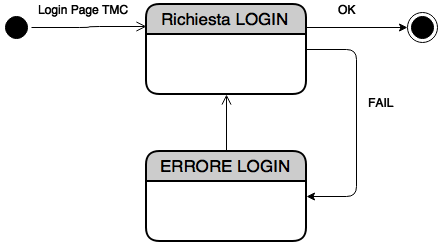
\includegraphics[scale=0.7]{Login.png}
\end{center}
\subsubsection{Precondizioni}
Nessuna.
\subsubsection{Assunti all'uscita}
Se il login va a buon fine, l'utente può accedere all'area riservata del sito con i privilegi che gli spettano(Amministratore o Regular).

\pagebreak

\subsection{Logout}
\subsubsection{Descrizione}
L'utente può effettuare il logout da qualunque pagina, a parte le pagine di errore e quelle di login. Premendo sul tasto dedicato, si viene indirizzati nuovamente alla pagina di login del sito.
\subsubsection{Diagramma di flusso}

\begin{center}
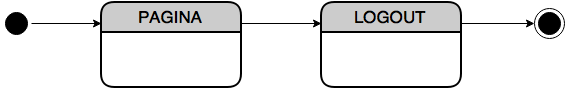
\includegraphics[scale=0.65]{Logout.png}
\end{center}
\subsubsection{Precondizioni}
L'utente deve essere regolarmente loggato all'interno del sito.
\subsubsection{Assunti all'uscita}
L'utente non risulta più loggato all'interno della propria area riservata sul sito.

\pagebreak

\section{Funzioni Regular}
Le funzioni di un regular user riguardano la consultazione di informazioni relative al veicolo tracciato, come schematizzato in seguito.
\begin{center}
\begin{tikzpicture}
\tikzumlset{fill usecase=white!10}

\umlusecase[x=2, y=-3.5, width=5cm]{Visualizza posizione}
\umlusecase[x=2, y=-5, width=5cm]{Controllo Eccesso Velocità}
\umlusecase[x=2, y=-6.5, width=5cm]{Consultazione Storico Furti}
\umlusecase[x=2, y=-8, width=5cm]{Live Tracking}



\umlactor[x=-6, y=-6.5, scale=1.5]{Regular}
\umlassoc{Regular}{usecase-5}
\umlassoc{Regular}{usecase-6}
\umlassoc{Regular}{usecase-7}
\umlassoc{Regular}{usecase-8}


\end{tikzpicture}
\end{center}

\subsection{Visualizza Posizione}
\subsubsection{Descrizione}
Accedendo al sito di TrackMyCar si possono consultare numerose informazioni riguardo il proprio veicolo, previo login. La pagina che viene restituita contiene una serie di operazioni svolgibili, di competenza dell'utente con privilegi non elevati. Selezionando la voce ``Posizione Veicoli'' si può verificare l'esatta ubicazione dei propri mezzi all'istante desiderato. Tale informazione viene segnalata su una mappa tramite un indicatore di posizione. 

In ogni momento si verifica se l'utente ha i privilegi necessari per accedere ad una determinata funzione, altrimenti viene indirizzato alla pagina di errore. Successivamente viene inviato alla propria home oppure alla pagina di login, secondo i casi.
\subsubsection{Diagramma di flusso}

\begin{center}
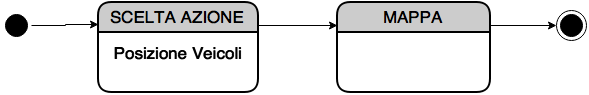
\includegraphics[scale=0.62]{Posizione.png}
\end{center}
\subsubsection{Precondizioni}
L'utente deve essere regolarmente loggato all'interno del sito e gli eventuali veicoli devono essere correttamente registrati.
\subsubsection{Assunti all'uscita}
Nessuno.

%\pagebreak

\subsection{Controllo Eccesso di Velocità}
\subsubsection{Descrizione}
Scegliendo la funzione associata è possibile consultare gli eventuali allarmi provocati dai veicoli a cui l'utente è legato. Nel caso non fosse associato alcun veicolo all'utente, tale evento verrà segnalato tramite un messaggio. 

\subsubsection{Diagramma di flusso}

\begin{center}
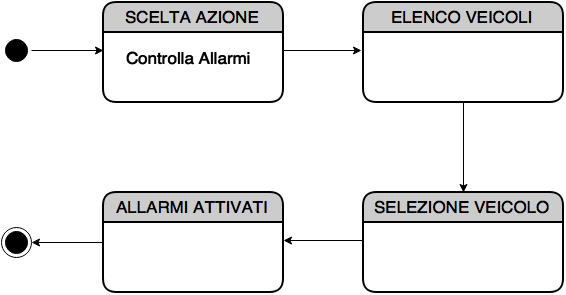
\includegraphics[scale=0.65]{Allarmi.png}
\end{center}
\subsubsection{Precondizioni}
L'utente deve essere regolarmente loggato all'interno del sito ed avere dei veicoli associati, nonchè degli allarmi impostati.
\subsubsection{Assunti all'uscita}
Nessuno.

\pagebreak

\subsection{Consultazione Storico Furti}
\subsubsection{Descrizione}
Funzione che, come da titolo, permette di tenere traccia degli eventuali furti ai danni dei veicoli associati all'utente. Dalla lista puntata, selezionando un furto, è possibile visualizzare a schermo la mappa del percorso effettuato durante la fuga del ladro. Nel caso non fosse associato alcun veicolo all'utente, tale evento verrà segnalato tramite un messaggio.
\subsubsection{Diagramma di flusso}

\begin{center}
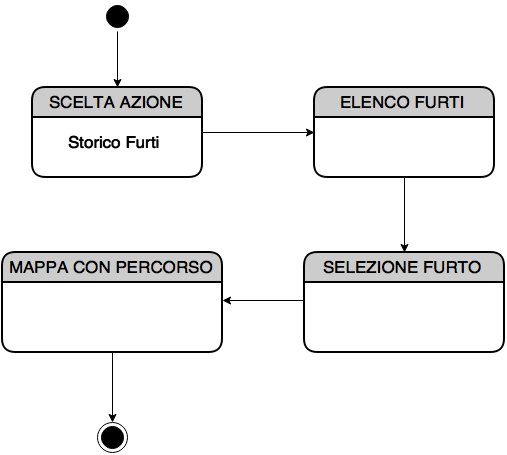
\includegraphics[scale=0.5]{Storico.png}
\end{center}
\subsubsection{Precondizioni}
L'utente deve essere regolarmente loggato all'interno del sito e deve avere veicoli associati.
\subsubsection{Assunti all'uscita}
Nessuno.

\pagebreak

\subsection{Live Tracking}
\subsubsection{Descrizione}
Selezionando la voce associata è possibile visualizzare tramite il proprio browser (in tempo reale) il percorso del veicolo scelto. All'interno della stessa pagina è possibile riprodurre in streaming il video del ladro direttamente dall'abitacolo. Nel caso l'utente non disponga di veicoli o non sia stato derubato, l'applicazione fornirà notifica a video.
\subsubsection{Diagramma di flusso}

\begin{center}
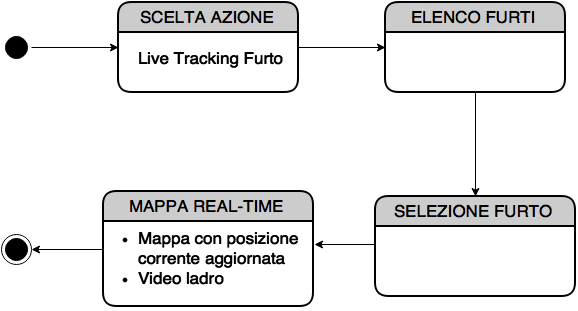
\includegraphics[scale=0.7]{Tracking.png}
\end{center}
\subsubsection{Precondizioni}
L'utente deve essere regolarmente loggato all'interno del sito e deve avere veicoli associati.
\subsubsection{Assunti all'uscita}
Nessuno.

\pagebreak

\section{Funzioni Amministratore}
Un amministratore gestisce i dati relativi agli utenti, ai gruppi ed alle funzioni ed i permessi ad operare. Può inoltre gestire l'associazione dei veicoli ai rispettivi utilizzatori, gli allarmi e le notifiche via SMS e mail. Tutte le funzioni disponibile per il Regular possono comunque essere svolte dall'amministratore.
\begin{center}
\begin{tikzpicture}
\tikzumlset{fill usecase=white!10}

\umlusecase[x=2, y=4, width=5cm]{Gestione Utenti}
\umlusecase[x=2, y=2.5, width=5cm]{Gestione Veicoli}
\umlusecase[x=2, y=1, width=5cm]{Associazione Guidatore-Veicolo}
\umlusecase[x=2, y=-0.5, width=5cm]{Impostazione Allarmi}


\umlactor[x=-6, y=1, scale=1.5]{Amministratore}
\umlassoc{Amministratore}{usecase-1}
\umlassoc{Amministratore}{usecase-2}
\umlassoc{Amministratore}{usecase-3}
\umlassoc{Amministratore}{usecase-4}


\end{tikzpicture}
\end{center}

\subsection{Gestione Utenti}
\subsubsection{Descrizione}
Attraverso la scelta di questa funzione, l'amministratore può decidere di operare sugli utenti che sfruttano l'applicazione. Le azioni disponibili permettono di aggiungere una nuova utenza, modificarne una esistente oppure eliminarla. Le ultime due funzioni presuppongono la scelta di un profilo da una lista, limitando così la possibilità di errori o incomprensioni per l'utilizzatore finale. La presenza di un amministratore è obbligatoria e non è possibile eliminarlo, in caso sia l'ultimo utente rimasto.
\subsubsection{Diagramma di flusso}

\begin{center}
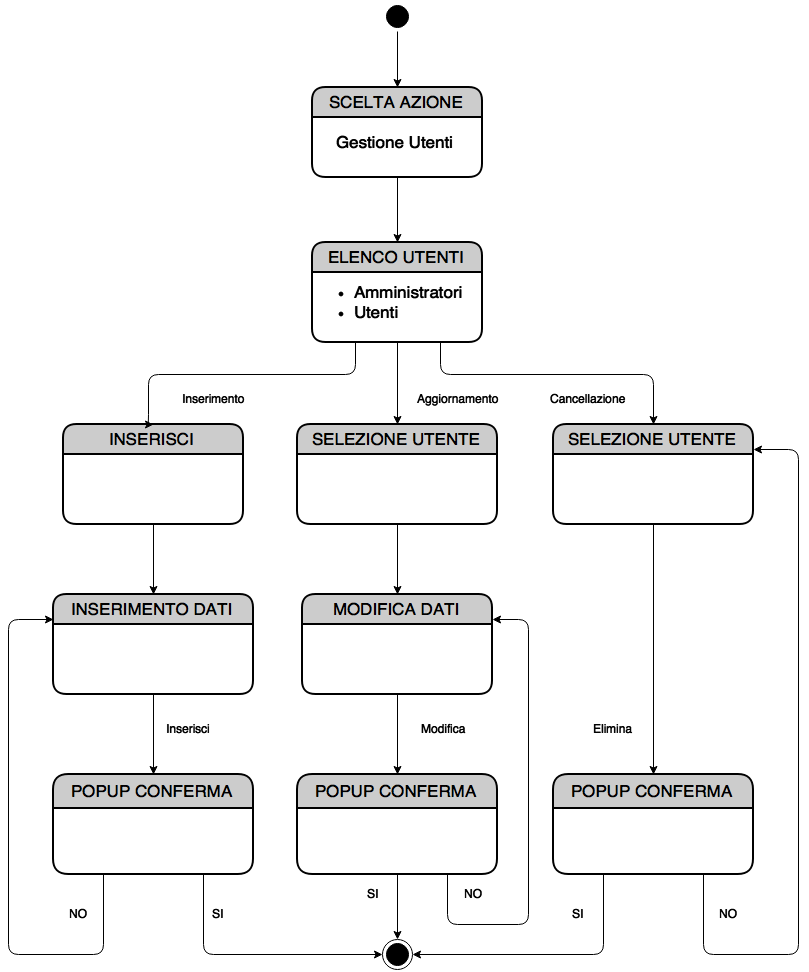
\includegraphics[scale=0.45]{Utenti.png}
\end{center}
\subsubsection{Precondizioni}
L'utente deve essere regolarmente loggato all'interno del sito, avendo privilegi di amministratore.
\subsubsection{Assunti all'uscita}
Nessuno.


\subsection{Gestione Veicoli}
\subsubsection{Descrizione}
La selezione di questa funzione permette all'utente di aggiungere o modificare/eliminare un veicolo all'interno della lista. L'elenco dei veicoli e i pulsanti sottostanti permettono di guidare l'utente nella scelta delle operazioni da compiere. Nel caso non siano presenti veicoli, l'utente verrà immediatamente informato da un messaggio a video.


\subsubsection{Diagramma di flusso}

\begin{center}
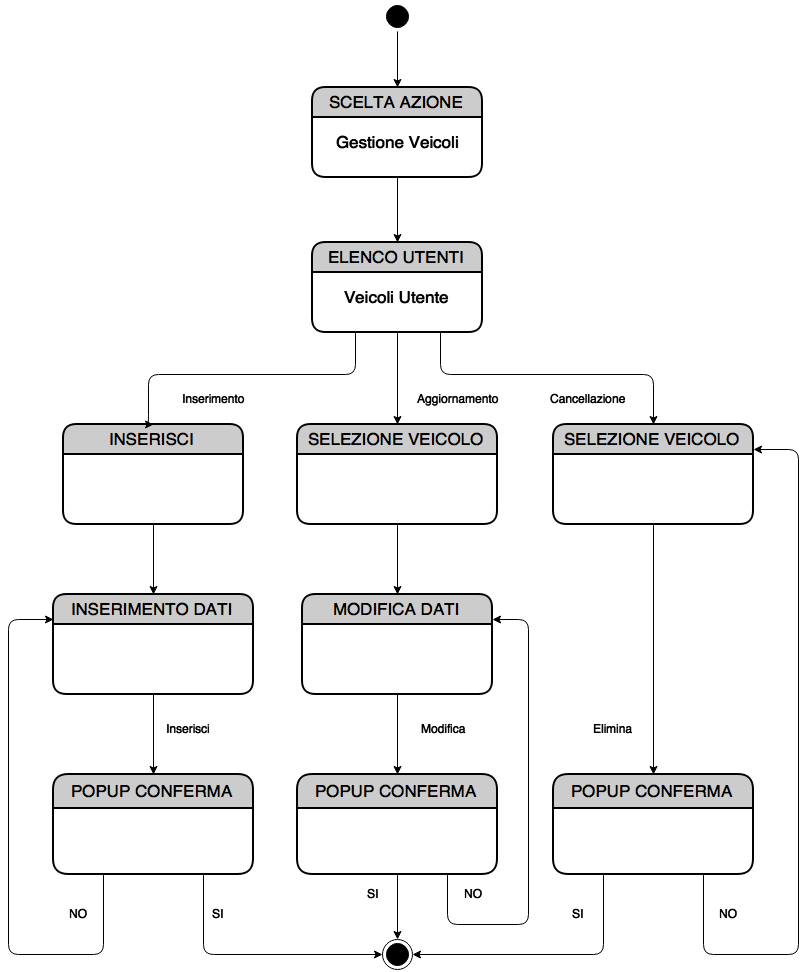
\includegraphics[scale=0.4]{Veicoli.png}
\end{center}
\subsubsection{Precondizioni}
L'utente deve essere regolarmente loggato all'interno del sito, avendo privilegi di amministratore. Devono esistere dei veicoli nel sistema.
\subsubsection{Assunti all'uscita}
Nessuno.



\subsection{Associazione Guidatore-Veicolo}
\subsubsection{Descrizione}
La pagina che viene mostrata selezionando la suddetta funzione permette di associare utenti e veicoli presenti nella base di dati. Nel caso non vi siano veicoli, l'utente verrà messo a conoscenza di ciò tramite un messaggio. Non è possibile che non siano presenti utenti da associare per quanto detto in precedenza (vedere Gestione Utenti).
\subsubsection{Diagramma di flusso}

\begin{center}
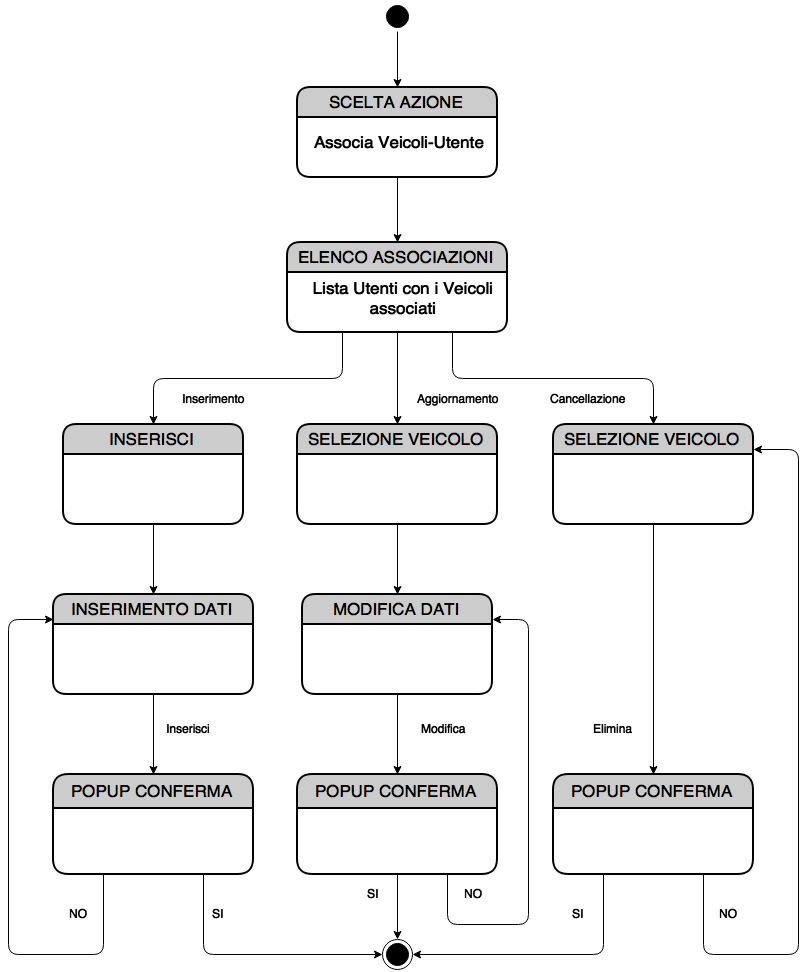
\includegraphics[scale=0.45]{Associa.png}
\end{center}
\subsubsection{Precondizioni}
L'utente deve essere regolarmente loggato all'interno del sito, avendo privilegi di amministratore. Devono esistere dei veicoli nel sistema.
\subsubsection{Assunti all'uscita}
Nessuno.

\pagebreak

\subsection{Impostazione Allarmi}
\subsubsection{Descrizione}
Scegliendo ``Imposta limite'' dalla pagina del profilo di amministratore, si viene diretti nella pagina di impostazione dei limiti a cui far scattare gli allarmi per eccesso di velocità. Tale funzione può essere espletata scegliendo un veicolo dalla lista e premendo su uno dei due tasti sottostanti la lista. Scegliendo la modifica, il limite verrà reimpostato (di default è 130 Km/h, impostato automaticamente in fase di inserimento di un nuovo veicolo), altrimenti questo può essere azzerato, eliminando le future notifiche agli utenti associati ai veicoli interessati.


\subsubsection{Diagramma di flusso}

\begin{center}
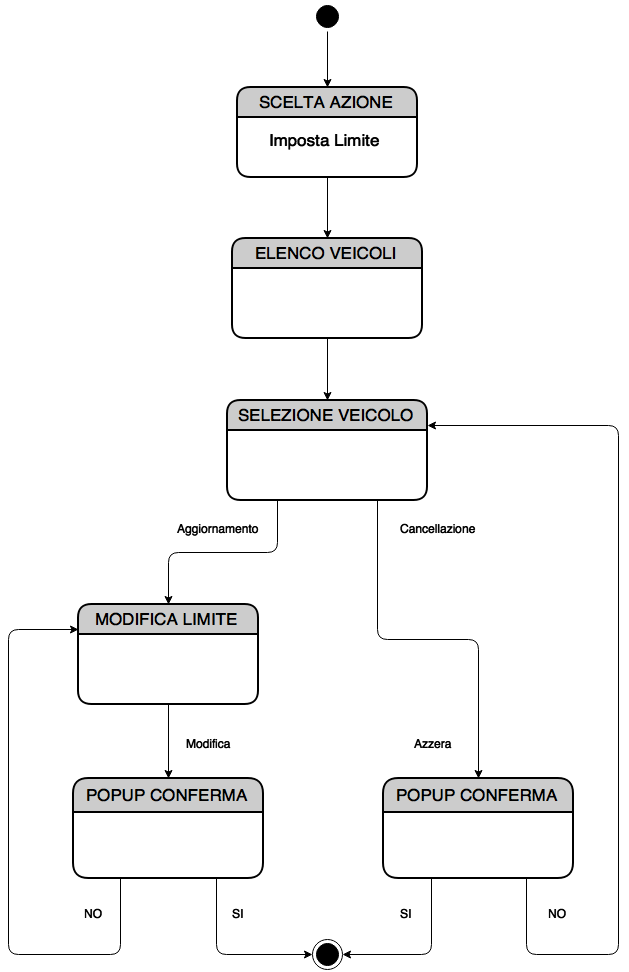
\includegraphics[scale=0.4]{Limite.png}
\end{center}
\subsubsection{Precondizioni}
L'utente deve essere regolarmente loggato all'interno del sito, avendo privilegi di amministratore. Devono esistere dei veicoli nel sistema.
\subsubsection{Assunti all'uscita}
Nessuno.

\pagebreak

\end{document}
